% "Станет проще"

\documentclass[12pt]{article}

% report, book

%  Русский язык

\usepackage[T2A]{fontenc}
\usepackage[utf8]{inputenc}
\usepackage[english,russian]{babel}

\usepackage{geometry}
\geometry{a4paper}

\usepackage{amsmath,amsfonts,amssymb,amsthm,mathtools} 

\usepackage{graphicx}


\usepackage{wasysym}

\usepackage{geometry} 
\geometry{a4paper,top=2cm,bottom=3cm,left=2cm}



\begin{document} % начало документа

\newpage

\section{Система Лоренца}
Об объекте можно говорить, как о динамической системе, если можно указать такой набор величин, называемых динамическими переменными и характеризующих состояние системы, что их значения в любой последующий момент времени получаются из исходного набора по определенному правилу.

Хоть и по определению динамической системы всегда можно однозначно предсказать конечное состояние по исходному, но в ней все равно может возникать хаос. В хаотическом режиме любая неточность в задании начального состояния нарастает во времени, так что предсказуемость становится недостижимой на достаточно больших интервалах времени. Такого рода режимы характеризуются нерегулярным, хаотическим изменением динамических переменных во времени.

Аттрактор Лоренца ― \textbf{компактное инвариантное множество} L в трехмерном фазовом пространстве гладкого потока. Система уравнений имеет вид
$$\begin{cases}	
	\dot{x} = \sigma (y-x) \\
	\dot{y} = x(\rho-z)-y \\
	\dot{z} = xy-bz
\end{cases}$$

Эта модель была впервые описана в 1963 году Эдвардом Лоренцом в статье "Детерминированное непериодическое течение". Лоренц получил эту модель как линейную аппроксимацию гидродинамической системы уравнений для задачи о конвекции морской воды в плоском слое; значения параметров и начальные условия были выбраны таким образом: $\sigma = 10$, $\rho = 28$, $b = \frac{8}{3}$; $x(0) = 1$, $y(0) = 0$, $z(0) = 0$.

Модель Лоренца является реальным физическим примером динамических систем с хаотическим поведением, в отличие от различных искусственно сконструированных отображений.

\section{Конвекция в замкнутой петле}

Трубка, замкнутая в кольцо, наполнена почти несжимаемой жидкостью. Она подогревается снизу и охлаждается сверху, и при достаточно сильном нагреве возможно возникновение конвекционного течения.

\begin{figure}[h]
	\centering
 	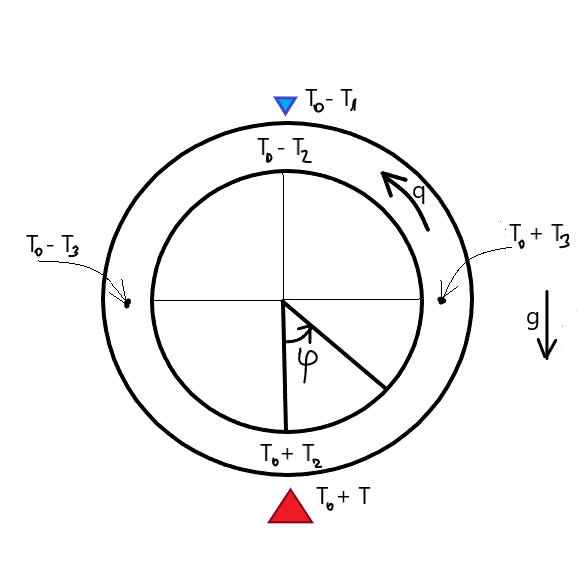
\includegraphics[scale=0.365]{Lorenz.png}
 	\caption{Кольцо с подогревом.}
\end{figure}

Пусть $a$ -- радиус петли, внутренний радиус много меньше $a$.

Заметим, что раз жидкость почти несжимаемая, то ее скорость во всех точках трубки постоянна, она не зависит от $\phi$. Обозначим скорость за $q = q(t)$.

Температура жидкости в трубке будет зависить от угла $\phi$, который отсчитывается от направленного вниз радиуса до точки против часовой стрелки. $T = T(\phi) -$ периодическая функция (период равен $2\pi$) $\Rightarrow$ ее можно разложить в ряд Фурье.

При разложении основную амплитуду задают первые слагаемые, поэтому рассмотрим только первую гармонику. Уравнение будет иметь вид 
\begin{equation}\label{eq1}
T - T_0 = T_2\cos\phi + T_1\sin\phi
\end{equation}
Исследуем коэффициенты при $\sin\phi$ и $\cos\phi$.

Рассмотрим $\phi = 0$ и $\phi = 2 \pi$, тогда $\cos\phi = 1, \sin\phi = 0$. Значит, $2T_2$ показывает разницу температур между нижней точкой (точка нагрева) и верхней точкой (точка охлаждения). Аналогично исследуем при $\phi = \frac{\pi}{2}$ и $\phi = \frac{3 \pi}{2}$. Получается, что $2T_3$ отвечает за разницу между боковыми точками петли. $T_2$ и $T_3$ зависят от времени.

Уравнение Навье-Стокса в общем виде:

\begin{equation*}
\frac{\partial \overrightarrow{u}}{\partial t} + \overrightarrow{u} \cdot \overrightarrow{\nabla} \overrightarrow{u} = -\frac{1}{\rho} \overrightarrow{\nabla} p - \overrightarrow{g} \alpha \Delta T + v \nabla^2 \overrightarrow{u}
\end{equation*}

В наших обозначениях:
\begin{itemize}
\item $\overrightarrow{u} \rightarrow q$
\item так как $q=q(t)$, то можно заменить $\frac{\partial q}{\partial t}$ на $\frac{dq}{dt}$
\item жидкость несжимаемая, следовательно $\overrightarrow{u} \cdot \overrightarrow{\nabla} \overrightarrow{u} \rightarrow 0$
\item при переходе в полярные координаты $\overrightarrow{\nabla} p \rightarrow \frac{1}{a} \frac{\partial p}{\partial \phi}$
\item действует сила Архимеда, она зависит от $\sin\phi$, следовательно $-\overrightarrow{g} \alpha \Delta T = g \alpha (T-T_0) \sin\phi$
\item коэффициент кинематической вязкости $\Gamma$ зависит от скорости, поэтому $v \nabla^2 \overrightarrow{u} \rightarrow -\Gamma q$
\end{itemize}

В итоге, уравнение Навье-Стокса для нашей системы примет вид:

\begin{equation}\label{eq2}
\frac{\partial q}{\partial t} = -\frac{1}{\rho a}\frac{\partial p}{\partial \phi} + g \alpha (T-T_0) \sin\phi -\Gamma q
\end{equation}

Подставим уравнение (\ref{eq1}) в (2):

\begin{equation*}
\frac{\partial q}{\partial t} = -\frac{1}{\rho a}\frac{\partial p}{\partial \phi} + g \alpha (T_2\cos\phi + T_1\sin\phi) \sin\phi -\Gamma q
\end{equation*}

Избавимся от части с давлением, проинтегрировав один раз от 0 до $2\pi$. Тогда 

\begin{equation*}
-\frac{1}{\rho a} \int_{0}^{2\pi} \frac{\partial p}{\partial \phi}\, d\phi = 0
\end{equation*}

\begin{equation*}
g \alpha T_2 \int_{0}^{2\pi} \cos\phi \sin\phi\, d\phi = \frac{1}{2} \sin^2 \phi \Big|_0^{2\pi} = 0
\end{equation*}

\begin{equation*}
g \alpha T_3 \int_{0}^{2\pi} \sin^2 \phi\, d\phi = g \alpha T_3 \pi
\end{equation*}

\begin{equation*}
\int_{0}^{2\pi} \frac{\partial q}{\partial t}\, d\phi = 2\pi
\end{equation*}

\begin{equation*}
\int_{0}^{2\pi} -\Gamma q\, d\phi = -2\pi\Gamma q
\end{equation*}

Тогда, поделив обе части уравнения на $2\pi$, получим:

\begin{equation}\label{eq23}
\frac{dq}{dt} = -\Gamma q + \frac{g \alpha T_3}{2}
\end{equation}

Таким образом, можно заметить, что скорость изменяется из-за разницы температур в боковых точках, то есть зависит от $2T_3$.

Теперь рассмотрим уравнение распространения теплоты в жидкости:

\begin{equation*}
\frac{\partial T}{\partial t} + \overrightarrow{u} \overrightarrow{\nabla} T = \kappa \nabla^2 T 
\end{equation*}
где $\kappa$ -- коэффициент температуропроводности.

В условиях задачи:

\begin{equation}\label{eq3}
\frac{\partial T}{\partial t} + \frac{q}{a} \frac{\partial T}{\partial \phi} = K(T_{external}-T_{internal}) = K(T_E-T)
\end{equation}

Внешняя температура зависит от высоты: 
\begin{equation}\label{eq4}
T_E = T_0+T_1\cos\phi
\end{equation}
Внутренняя же температура зависит от $T_2$ и $T_3$ (уравнение (\ref{eq1})). Вычтем из (\ref{eq1}) (4) и подставим в (3):

\begin{equation*}
\frac{dT_2}{dt}\cos\phi + \frac{dT_3}{dt}\sin\phi - \frac{q}{a}T_2\sin\phi + \frac{q}{a}T_3\cos\phi = K(T_1-T_2)\cos\phi-KT_3\sin\phi
\end{equation*}

Коэффициенты при $\sin\phi$ и $\cos\phi$ должны совпадать в обеих частях, следовательно 

\begin{equation*}
\frac{dT_3}{dt} - \frac{qT_2}{a} = -KT_3
\end{equation*}

\begin{equation*}
\frac{dT_2}{dt} + \frac{qT_3}{a} = K(T_1-T_2) = KT_4
\end{equation*}
где $T_4$ показывает разницу внешней и внутренней температуры внизу и вверху трубки.

\begin{equation}\label{eq5}
\frac{qT_2}{a} = \frac{qT_1}{a} - \frac{qT_4}{a} \Longrightarrow \frac{dT_3}{dt} = -KT_3 + \frac{qT_1}{a} - \frac{qT_4}{a}
\end{equation}

$T_1$ определяется конфигурацией системы и не зависит от времени, следовательно, $\frac{dT_2}{dt} = -\frac{dT_4}{dt} \Longrightarrow$

\begin{equation}\label{eq6}
\frac{dT_4}{dt} = -KT_4 + \frac{qT_3}{a}
\end{equation}

Уравнения (3), (6) и (7) образуют систему дифференциальных уравнений, которую можно привести к виду системы Лоренца. Для этого сделаем следующие замены:
\begin{equation*}
q = aKx, \quad T_3 = \frac{2a \Gamma Ky}{g \alpha}, \quad T_4 = \frac{2a \Gamma Kz}{g \alpha}, \quad t \rightarrow Kt
\end{equation*}

Тогда

\begin{equation*}
aK^2\dot{x} = -\Gamma aKx + a\Gamma Ky \Longrightarrow \dot{x} = \frac{\Gamma}{K} (y - x)
\end{equation*}

\begin{equation*}
\frac{2a\Gamma K^2}{g\alpha} \dot{y} = -\frac{2a\Gamma K^2}{g\alpha}y + \frac{aKxT_1}{a} - \frac{aKx \cdot 2a \Gamma Kz}{ag\alpha} \Longrightarrow \dot{y} = -y + \frac{g\alpha T_1}{2a\Gamma K}x - xz
\end{equation*}

\begin{equation*}
\frac{2a\Gamma K^2}{g\alpha} \dot{z} = -\frac{K \cdot 2a\Gamma K}{g\alpha} + \frac{aKx \cdot 2a\Gamma Ky}{a} \Longrightarrow \dot{z} = -z+xy
\end{equation*}


Таким образом, была получена система дифференциальных уравнений Лоренца.
$$\begin{cases}	
	\dot{x} = \sigma (y-x) \\
	\dot{y} = x(\rho-z)-y \\
	\dot{z} = xy-bz
\end{cases}$$
где 
\[ \rho = \frac{g\alpha T_1}{2a\Gamma K} - \text{число Рэлея}\]
\[P = \frac{\Gamma}{K} - \text{число Прандтля}\] 

Число Релея определяет поведение жидкости под воздействием градиента температуры. Число Прандтля -- один из критериев подобия тепловых процессов в жидкостях, который учитывает флияние физических свойств теплоносителя на теплоотдачу.

В условиях данной задачи $x$ показывает скорость течения, $y$ -- отклонение температуры от средней в точке $\phi = \frac{\pi}{2}$, $z$ -- то же, но в нижней точке.

\section{Другие области применения}

Модель Лоренца применима в других физических процессах:
\begin{itemize}
	\item Конвекция в плоском слое
	\item Вращение водяного колеса (колесо, на ободе которого укреплены корзины с отверстиями в дне; сверху на колесо симметрично относительно оси вращения льётся сплошной поток воды)
	\item Одномодовый лазер
	\item Диссипативный осциллятор с инерционным возбуждением
\end{itemize}

При этом в других моделях переменные и параметры будут иметь другой смысл. Так для конвекции в плоском слое $x$ отвечает за скорость вращения водяных валов, $y$ и $z$ -- за распределение температуры по горизонтали и вертикали, $\rho$ -- нормированное число Рэлея, $\sigma$ -- число Прандтля (отношение коэффициента кинематической вязкости к коэффициенту температуропроводности), $b$ содержит информацию о геометрии конвективной ячейки. 

Вращение водяного колеса похоже по поведению на конвецкцию в замкнутой петле с точностью до переворота "вверх ногами", поэтому описывается аналогичными уравнениями с заменой температуры на плотность распределения массы воды в корзинах по ободу.

Для одномодового лазера $x$ -- амплитуда волн в резонаторе лазера, $y$ -- поляризация, $z$ -- инверсия населённостей энергетических уровней, $b$ и $\sigma$ -- отношения коэффициентов релаксации инверсии и поля к коэффициенту релаксации поляризации, $\rho$ -- интенсивность накачки.


\end{document} % конец документа